\documentclass[a4paper,oneside,11pt]{book}

%~ language : load french support
\usepackage[frenchb]{babel} 
\usepackage[T1]{fontenc}
\usepackage[utf8]{inputenc} 

% !TEX ../report.tex

%~ paper and margins
\usepackage[tmargin=2.2cm,bmargin=2.2cm,lmargin=2.5cm,rmargin=2.5cm]{geometry}
\setlength{\parindent}{0pt} % no indent
\setlength{\parskip}{\baselineskip} % bare line between paragraphs
\setlength{\baselineskip}{2.5pt}


%~ section headings : decrease the spaces above and below
\usepackage{titlesec}
\titlespacing\section{0pt}{2pt plus 1pt minus 2pt}{-4pt plus 2pt minus 2pt}
\titlespacing\subsection{0pt}{2pt plus 1pt minus 2pt}{-4pt plus 2pt minus 2pt}
\titlespacing\subsubsection{0pt}{2pt plus 1pt minus 2pt}{-4pt plus 2pt minus 2pt}

%~ add default spaces between items in lists
\usepackage{enumitem}
\setitemize{itemsep=3pt}


% hyperref setup
\usepackage[colorlinks=true,urlcolor=blue!30!black,linkcolor=blue!30!black,urlbordercolor={1 0 0},pdfborder=0]{hyperref}

%~ graphics
\usepackage{graphicx} % for images
\graphicspath{{resources/}}
\usepackage{float}


%~ other really useful packages
\usepackage{tabularx}
\usepackage{amsmath,amsfonts,amsthm,amssymb}
\usepackage[usenames,dvipsnames,svgnames,table]{xcolor}

% --------------------------------------------------------------------------
% ADDITIONAL PACKAGES
% --------------------------------------------------------------------------

%~landscape support
\usepackage{pdflscape}

% --------------------------------------------------------------------------
% MINITOR
% --------------------------------------------------------------------------

%% minitoc setup
\usepackage{minitoc}
\renewcommand{\mtctitle}{}   % no title
\setcounter{minitocdepth}{1} % only \section
\nomtcrule                   % remove default black rules (we will add ours with \myminitoc)

% add gray rules to the minitoc top-bottom
\newcommand{\myminitoc}{
    \vspace{-1cm}
    {\hspace{8mm}\Large\emph{Contenu du chapitre}}
    {\color{light-gray}\hrule}
    \minitoc
    {\color{light-gray}\hrule}
    \vspace{.5cm}
}
% ------------------------------------------------------------------------------
% Set cool chapter titles
% ------------------------------------------------------------------------------

%Options: Sonny, Lenny, Glenn, Conny, Rejne, Bjarne, Bjornstrup
\usepackage[Bjornstrup]{fncychap}
\ChTitleVar{\raggedleft \huge\fontfamily{pzc}\selectfont}
%moins d'espace avant un chapitre
\makeatletter
\renewcommand*{\@makechapterhead}[1]{%
  \vspace*{0\p@}%
  {\parindent \z@ \raggedright \normalfont 
    \ifnum \c@secnumdepth >\m@ne
      \if@mainmatter%%%%% Fix for frontmatter, mainmatter, and backmatter 040920
        \DOCH
      \fi
    \fi
    \interlinepenalty\@M
    \if@mainmatter%%%%% Fix for frontmatter, mainmatter, and backmatter 060424
      \DOTI{#1}%
    \else%
      \DOTIS{#1}%
    \fi
  }}
% For the case \chapter*:
\renewcommand*{\@makeschapterhead}[1]{%
  \vspace*{0\p@}%
  {\parindent \z@ \raggedright
    \normalfont
    \interlinepenalty\@M
    \DOTIS{#1}
    \vskip 40\p@
  }}
\makeatother

% --------------------------------------------------------------------------
% TABLES
% --------------------------------------------------------------------------

\usepackage{array}
\usepackage{booktabs}

\renewcommand{\arraystretch}{1.2} % more space between rows 

%~ cellhead{align}{text}
\newcommand{\cellhead}[2]{\multicolumn{1}{#1}{\textbf{#2}}}

%~ use dotted or dash lines instead of solid ones
\usepackage{arydshln}
\setlength\dashlinedash{1pt}
\setlength\dashlinegap{1pt}
\setlength\arrayrulewidth{0.5pt}
\definecolor{light-gray}{gray}{0.92}
%~ \grayrule
\newcommand{\grayrule}{\arrayrulecolor{light-gray}\hdashline\arrayrulecolor{black}}

% --------------------------------------------------------------------------
% MINTED
% --------------------------------------------------------------------------
   
 \usepackage[outputdir="out"]{minted}
 \usemintedstyle{github}
 
 \newminted{prolog}{
     fontsize=\small, 
     xleftmargin=2mm,
     breaklines
 }
 
 \newminted{text}{
     fontsize=\small, 
     xleftmargin=2mm,
     breaklines
 }
 
 \newminted{java}{ 
      xrightmargin=2mm, 
      xleftmargin=2mm, 
      bgcolor=white,
      fontsize=\small
 }
 
 % repeat the command, since the minted package changes that
 \makeatletter 
 \renewcommand\verbatim@font{\footnotesize\ttfamily\color{black}}
 \makeatother
 
% --------------------------------------------------------------------------
% COMMANDS
% --------------------------------------------------------------------------

%~ \begin{dotitemize} 
%~ bulleted list 
\newcommand{\sbt}{\,\begin{picture}(-1,1)(-1,-3)\circle*{2.3}\end{picture}\ }
\newenvironment{dotitemize}{ 
    \begin{list}{$\sbt$}{
        \setlength\itemsep{2pt}
        \setlength\parindent{2pt}
        \setlength\labelsep{13pt}
    }
}{\end{list}}


%~ include a figure, centered, with caption and label
%~ usage : \includeFigure{percentage of textwidth}{path}{caption}
%~ requires \usepackage{float}
\newcommand{\includeFigure}[3]{
    \begin{figure}[H]
    \centering
    \includegraphics[width=#1\textwidth]{#2}
    \caption{#3}
    \label{fig:#2}
    \end{figure}
}

%~ \code[text]
%~ text in monospace font
\newcommand{\code}[1]{{\small\texttt{#1}\normalsize}}


%~ \guillemets[text] 
%~ enclose the text between french quotes
%\newcommand{\guillemets}[1]{\og#1\fg{}}
%~ enclose the texte between english quotes
\newcommand{\guillemets}[1]{``#1''}

%~ \begin{notepar}{title}
%~ \end{notepar}
%~ source: http://mirror.switch.ch/ftp/mirror/tex/macros/latex/contrib/tcolorbox/tcolorbox.pdf
\usepackage{tcolorbox}
\definecolor{light-gray}{gray}{0.85}
\definecolor{dark-gray}{gray}{0.10}
\newenvironment{notepar}[1]% 
  {\begin{tcolorbox}[title={#1},colback=white,colframe=light-gray,coltext=dark-gray,coltitle=dark-gray,fonttitle=\bfseries\large]}
  {\end{tcolorbox}}



\setcounter{secnumdepth}{4} % allows 4 numbered subsections 
% it is possible to use \paragraph for the 4th level

\newcommand{\easypass}{\emph{EasyPass}}
% --------------------------------------------------------------------------
% META
% --------------------------------------------------------------------------

%~ include title page command \lltitlepage
\usepackage{titling} % to have thetitle, theauthor, thedate available
% !TEX ../report.tex

%---------------------------------------------------------------------------
% CONFIG
%---------------------------------------------------------------------------

\newcommand{\institutionlogo}{logo_hesso}
\newcommand{\institutionlogowidth}{200px}
\newcommand{\institution}{}
\newcommand{\titleaboveone}{Mobile (MobOp)}
\newcommand{\titleabovetwo}{Mini projet}
\newcommand{\subtitle}{Passwords at your fingertips}
\newcommand{\logo}{logo.png}
\newcommand{\logowidth}{200px}

% \newcommand{\auteurs}{
%  \emph{Auteur~:}  Lucy \textsc{Linder}
%       %Second author ~\\[0.2cm]
% }

% ~ use this for multiple authors
\newcommand{\auteurs}{
\emph{Auteurs~:} \\[0.4cm]
     Lucy \textsc{Linder} ~\\[0.2cm]
     Magali \textsc{Froehlich} 
}

% \newcommand{\profs}{}
%~ use this for professors:
\newcommand{\profs}{
\emph{Professeur~:} \\[0.4cm]
     Pascal \textsc{Bruegger} ~\\[0.2cm]
     %Second prof ~\\[0.2cm]
}


%----------------------------------------------------------------------------
% TITLE 
%----------------------------------------------------------------------------

\newcommand{\HRule}[1]{\rule{\linewidth}{#1}}  

\newcommand{\lltitlepage}{
	\begin{titlepage}	
    \center
    %--- institution logo and name
    \begin{flushright}
    \ifdefempty{\institutionlogowidth}{
    	\includegraphics{\institutionlogo}
    }{
    	\includegraphics[width=\institutionlogowidth]{\institutionlogo}
    }
    \end{flushright}
    \ifdefempty{\institution}{~}{\textsc{\large \institution}} \\[2cm]
    %--- above the title: course name for example
    \ifdefempty{\titleaboveone}{}{\textsc{\Large \titleaboveone} ~\\[0.5cm]} 
    \ifdefempty{\titleabovetwo}{}{\textsc{\titleabovetwo} ~\\[0.5cm]} 

    %---  title inside rules
    \HRule{0.5mm} 
    \\[0.4cm]
    {\huge \bfseries \thetitle} % title
    \\[0.3cm] 
    \ifdefempty{\subtitle}{}{{\Large \subtitle}\\[0.3cm]} % subtitle
    \HRule{0.6mm} 
                
    % --- logo
    \ifdefempty{\logo}{}{
    	~\\[1cm]
    	\ifdefempty{\logowidth}{
			
\includegraphics{\logo}   		
    	}{
			
\includegraphics[width=\logowidth]{\logo}
    	}
    	\vfill
    }

    
    \ifdefempty{\profs}{
    	\begin{center} \large
    		\auteurs 
    	\end{center} 
    }{
	    % --- author(s) on the left
	    \begin{minipage}[t]{0.4\textwidth}
	    \begin{flushleft} \large
	     \auteurs     
	    \end{flushleft}
	    \end{minipage}
	    ~ % --- prof name on the right
	    \begin{minipage}[t]{0.4\textwidth} 
	    \begin{flushright} \large
	    	\profs
	    \end{flushright}
	    \end{minipage}
	}
    \vfill
    \thedate
    ~\\[2cm]
    
    \setcounter{page}{1}
	\end{titlepage}
} % end title command % include the title page

%~ metas
\title{EasyPass} % TODO
\author{Lucy Linder}
\date{01.01.2018} % TODO

%~ logo of the school in filigrane
\usepackage{wallpaper}
\newcommand{\llwallpaper}{filigrane-mse.pdf}
%~ use 

% --------------------------------------------------------------------------
% HEADER/FOOTER
% --------------------------------------------------------------------------

\usepackage{fancyhdr}
\usepackage{lastpage}

%% header/footer management

\pagestyle{fancy} % default style = fancy
\fancyhf{} % reinit

% set default header to `1. chapter name`, with hrule
\renewcommand{\chaptermark}[1]{\markboth{\thechapter.\ #1}{}}
\fancyhead[R]{\small\itshape\MakeUppercase{\leftmark}}
% set default footer to <name of school> -> 1/10 
\usepackage{lastpage}
\newcommand{\leftfootcontent}{\small\itshape{Master MSE, MobOp}}
\newcommand{\rightfootcontent}{\thepage\  / \pageref{LastPage}}
\renewcommand{\footrulewidth}{0.1pt}
\fancyfoot[R]{\rightfootcontent}
\fancyfoot[L]{\leftfootcontent}

% set style used by chapter/parts to footer only
\fancypagestyle{plain}{
  \renewcommand{\headrulewidth}{0pt}
   \renewcommand{\footrulewidth}{0.1pt} % default .4pt
  \fancyhf{}
  \fancyfoot[R]{\rightfootcontent}
  \fancyfoot[L]{\leftfootcontent}
}

% set style empty to nothing
\fancypagestyle{empty}{
  \renewcommand{\headrulewidth}{0pt}
   \renewcommand{\footrulewidth}{0pt} % default .4pt
  \fancyhf{}
}

% --------------------------------------------------------------------------
% TOC
% --------------------------------------------------------------------------

%~ toc
\usepackage{tocloft}
%~ change toc title (with babel french package)
\addto\captionsfrench{\renewcommand\contentsname{Table of Contents}}

% --------------------------------------------------------------------------
% CONTENT
% --------------------------------------------------------------------------

\begin{document} 

%--- toc
\dominitoc % Initialization of minitoc out of the block !
{   
    % in here, no header/footer
    \pagestyle{empty}

    \lltitlepage
    \cleardoublepage

    \ULCornerWallPaper{1}{\llwallpaper}
    \tableofcontents
    \cleardoublepage
}
% ------------------------------------ document

\setcounter{page}{1} % first numbered page
\chapter{Introduction}\label{chap:intro}
%\myminitoc
% !TEX ../report.tex

Ce rapport présente l'application Android \easypass{} conçue dans le cadre du cours MSE \guillemets{MobOp}. 

\section{Concept}

\easypass{} est une application de gestion de mots de passe. 

Tout comme ses concurrents (\emph{LastPass}, etc.), il permet de stocker de manière sécurisée ses mots de passe et de les consulter depuis n'importe où au moyen d'un unique \emph{Master Password}. L'originalité et l'avantage d'\easypass{{} repose dans la manière dont il stocke les informations. 

\includeFigure{1}{intro}{Slides présentés au lancement de l'application. Un gradient de couleurs apparait lors du swipe.}

\emph{LastPass} par exemple possède ses propres serveurs, tandis que d'autres ont opté pour un stockage local, sur l'ordinateur de l'utilisateur. Dans le premier cas, il est nécessaire d'avoir une confiance totale dans les serveurs du service. Dans le second cas, un accident et nous perdons nos mots de passe (à moins de maitriser l'art de la sauvegarde, ce qui n'est pas si courant).

\easypass{} a opté pour une solution hybride: tous les mots de passe sont sauvegardés dans un simple fichier synchronisé sur \emph{Dropbox}. Ce dernier se charge d'en assurer les sauvegardes et tant qu'un ordinateur est lié au service, une copie locale existe également!

% Stocker des mots de passe sur \emph{Dropbox}... Est-ce sécurisé ? \\
Pour assurer la sécurité des mots de passe, le contenu du fichier est chiffré en utilisant l'algorithme de chiffrement AES~CBC~256. Cet algorithme est pour l'instant considéré comme \guillemets{strong}, mais a également un autre avantage: il est supporté par de nombreux logiciels, notamment \code{openssl}. Ainsi, même si \easypass{} est indisponible ou présente un bug, l'utilisateur peut à tout moment récupérer ses informations en tapant une simple ligne dans son terminal ou un autre outil de la suite \easypass.

% 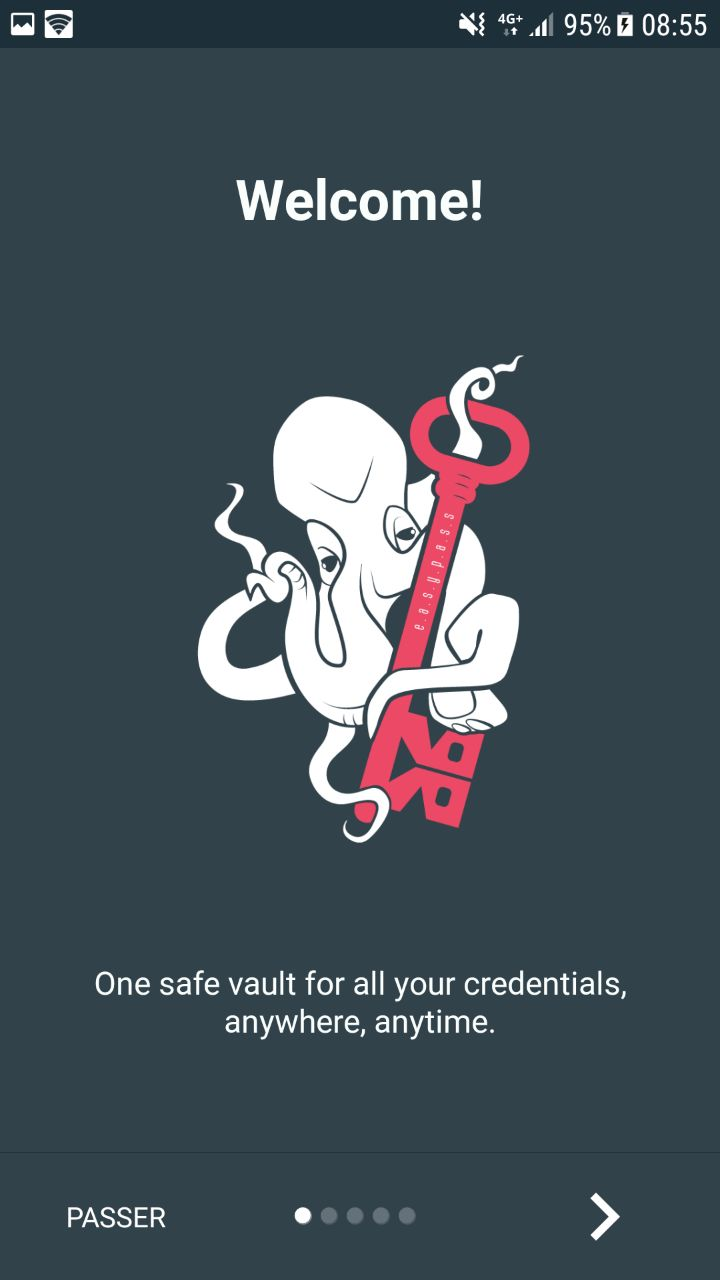
\includegraphics[width=.2\textwidth]{intro-1.jpg}
% 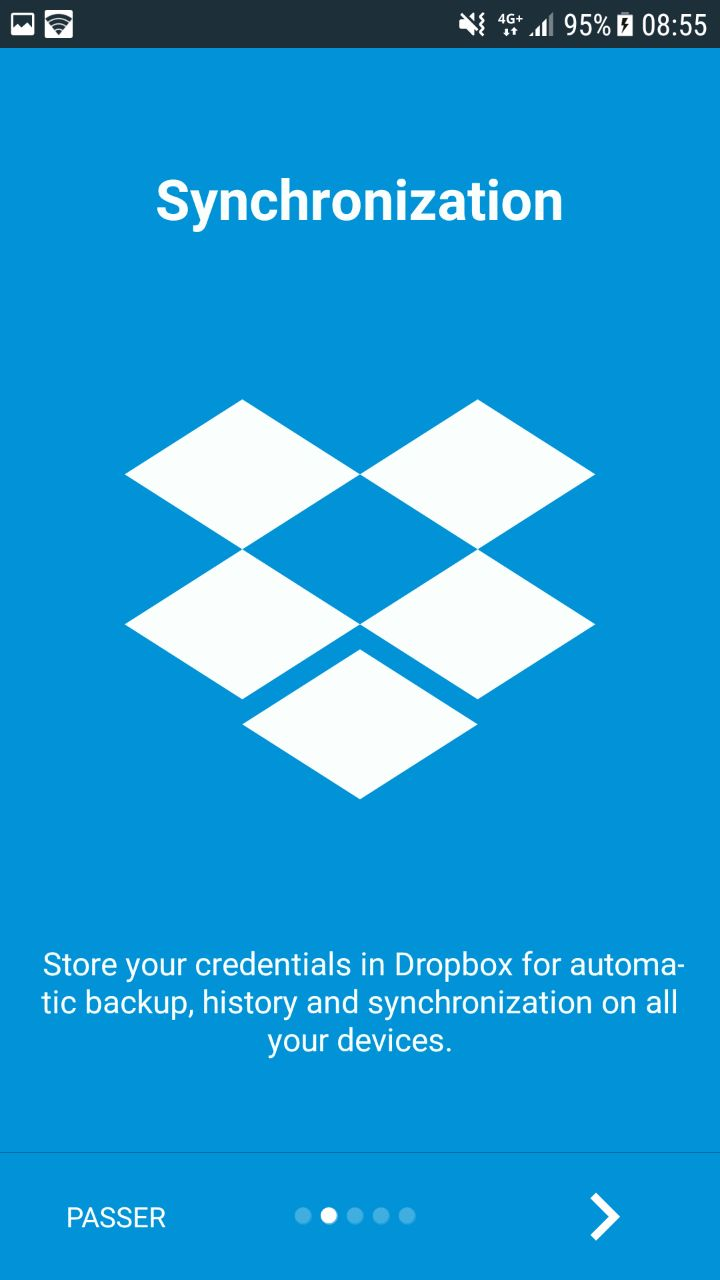
\includegraphics[width=.2\textwidth]{intro-2.jpg}
% 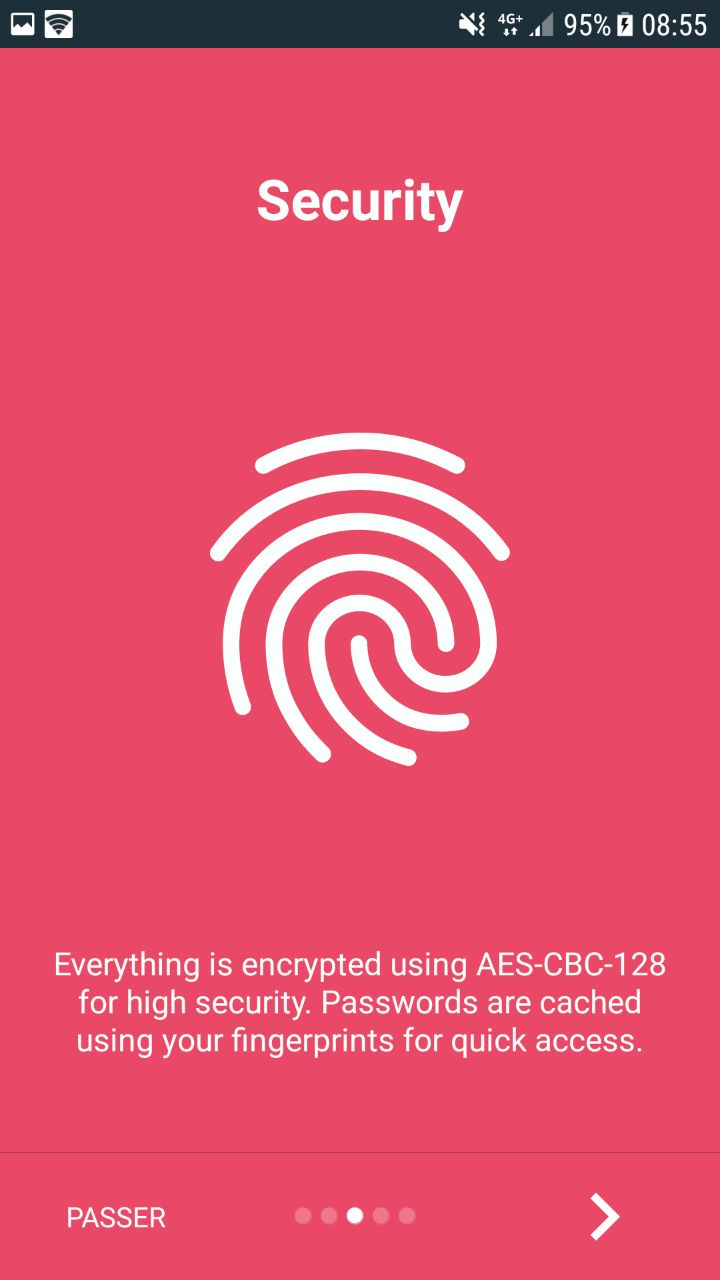
\includegraphics[width=.2\textwidth]{intro-3.jpg}
% 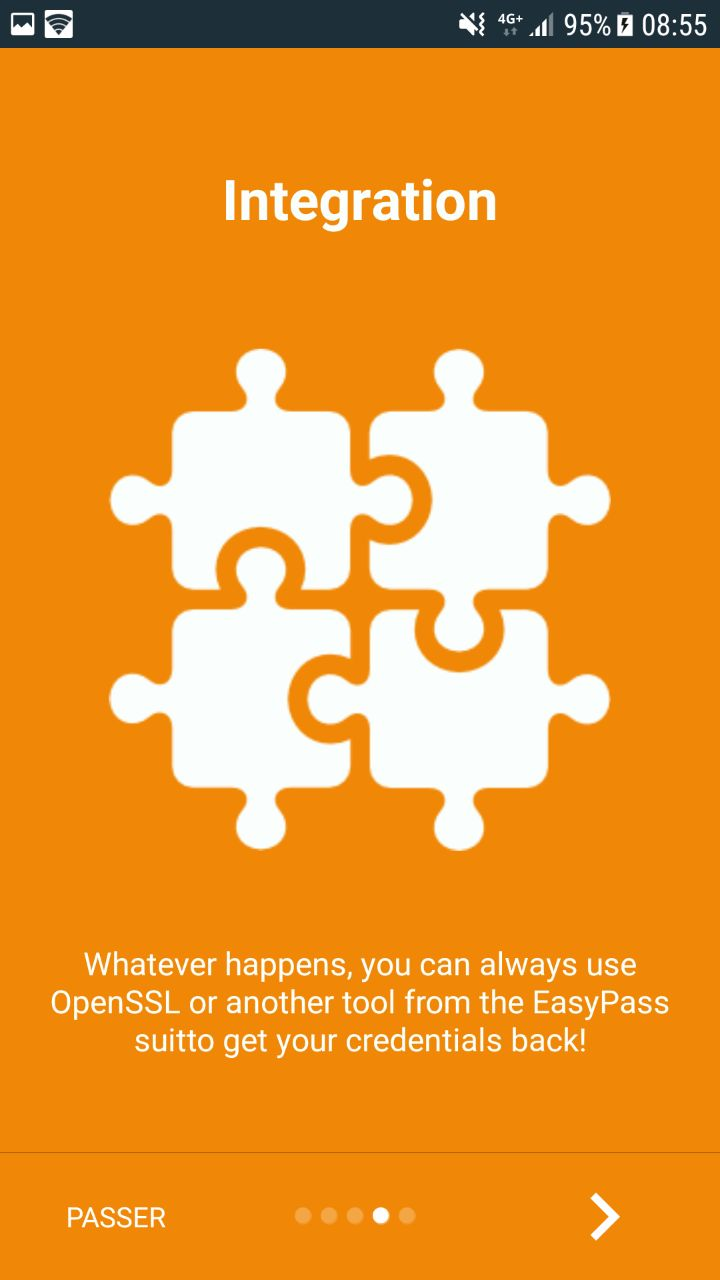
\includegraphics[width=.2\textwidth]{intro-4.jpg}
% 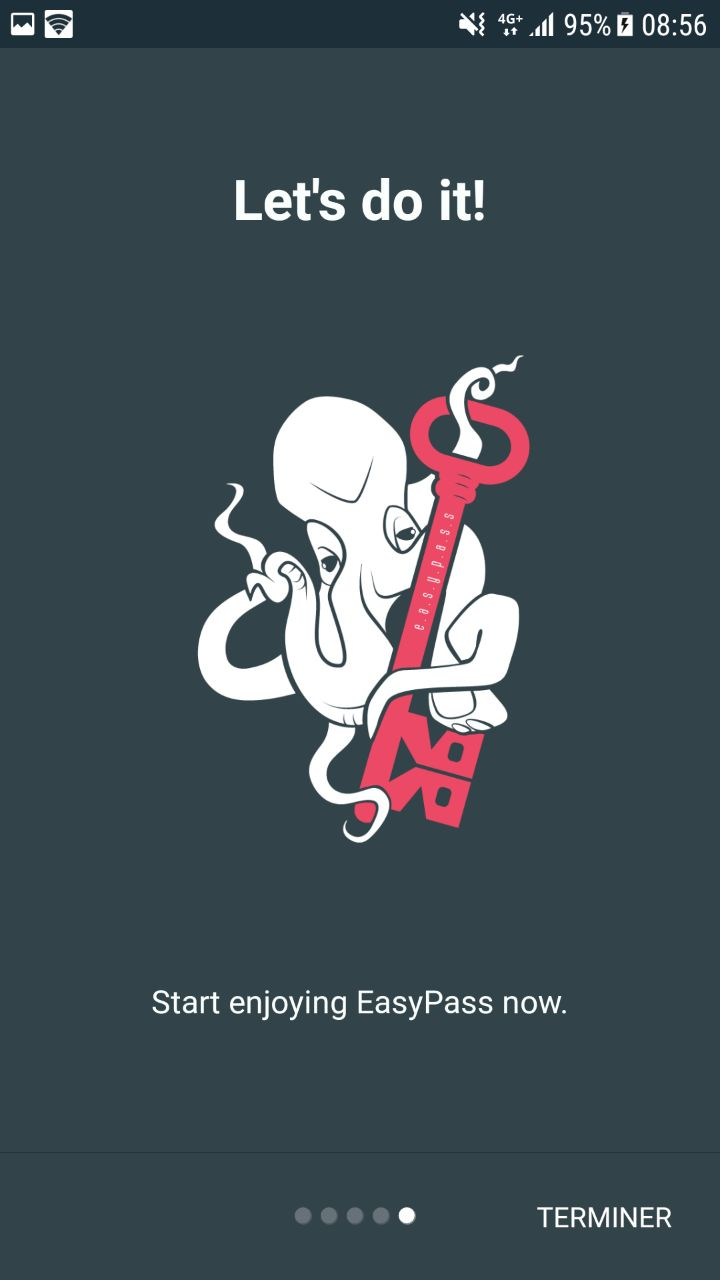
\includegraphics[width=.2\textwidth]{intro-5.jpg}



\section{Vocabulaire}

Dans ce document, nous utiliserons les termes suivants:

\begin{description}
    \item[compte/account] un ensemble d'information concernant un mot de passe: nom, email, pseudo, notes, date de création, date de modification;
    \item[session] un fichier contenant un ensemble de comptes, sécurisé par un mot de passe unique;
    \item[master password] un mot de passe permettant de décrypter une session.
\end{description}


% Fonctionnalités de base:

% \begin{itemize}
%     \item liste des comptes (une seule session);
%     \item opérations CRUD sur un compte;
%     \item synchronisation de la session au format json sur Dropbox;
%     \item cryptage AES CBC de la session avec mot de passe;
%     \item décryptage de la session via \emph{fingerprint} ou \emph{pattern};
%     \item raccourcis pour copier rapidement une information de compte (mot de passe, email, pseudo);
%     \item fonctionnalité de recherche via mot-clés; 
% \end{itemize}

% Fonctionnalités optionnelles (\emph{nice to have}):

% \begin{itemize}
%     \item (implémenté) sécursation de l'application: pas de capture d'écran ni de preview dans les \emph{recents};
%     \item (implémenté) générateur de mot de passe;
%     \item historique des mots de passe pour un compte;
%     \item gestion des duplicats; 
%     \item feedbacks visuels concernant la sécurité des mots de passe: \emph{weak, OK, strong};
%     \item support d'autres plateformes que Dropbox (Google Drive, etc.);
%     \item portage sur IOS;
% \end{itemize}


\chapter{Présentation}\label{chap:presentation}
%\myminitoc
% !TEX ../report.tex

fonctionnalités et captures aussi sur tablette !

\chapter{Implémentation}\label{chap:implementation}
%\myminitoc
% !TEX ../report.tex

L'application \easypass{} fut développée en Kotlin (version 1.1.60).


\section{Composants et structure du projet}

L'application est composée de six activités (voir figure \ref{fig:app-structure}). Les deux activités principales sont l'activité présentant la liste des comptes (\code{AccountListActivity}) et l'activité (\code{AccountDetailActivity}) permettant de manipuler un compte (pas utilisée sur tablette). 
% Sur tablette, \code{AccountListActivity} comprend les fragments de manipulation d'un compte (\emph{two panes}, \code{AccountDetailActivity} n'est pas utilisé).

Nous avons utilisé des fragments dans deux cas: a) dans la \code{LoadingSessionActivity}, où chaque fragment représente une vue dans un \emph{wizard}, b) dans les vues principales afin de pouvoir créer une interface \emph{two-panes} sur tablette.

\includeFigure{1}{app-structure}{Aperçu: activités, navigation et composants principaux}

Le projet est structuré en trois \emph{packages}\footnote{Nous avons favorisé des noms clairs à une arborescence complexe.}:

\begin{itemize}
\item \code{ch.derlin.easypass} contient toutes les classes liées aux vues (activités, fragments et adapteurs de liste);
\item \code{ch.derlin.easypass.helper} regroupe des objets statiques/classes implémentant la logique applicative ainsi que des classes réutilisables dans d'autres projets;
\item \code{ch.derlin.easypass.data} contient les définitions des données (\emph{data classes}) ainsi que le gestionnaire de sérialisation.
\end{itemize}

\section{Dropbox}

\begin{notepar}{Note}
Dans sa version V1, l'API Dropbox mettait à disposition des \emph{native SDKs} pour Android, IOS, etc.\footnote{Voir \url{https://www.dropbox.com/developers-v1/sync/sdks/android}.} Le téléchargement et la synchronisation des fichiers étaient entièrement pris en charge, rendant notre travail de développement aisé. Depuis la mise en service de l'API REST V2, ces SDKs ne sont plus disponibles.
\end{notepar}

Dropbox met à disposition un Java SDK\footnote{url: \url{https://github.com/dropbox/dropbox-sdk-java}.}. Avant de l'utiliser, il faut enregister une nouvelle application dans le panel développeur de Dropbox et obtenir une Apikey. La procédure est gratuire, mais le nombre d'utilisateurs est limité. \\
Le SDK est moins bien documenté que sa version 1 et n'offre ni SDK, ni un tutoriel spécifique pour Android. Il faut se référer à un exemple officiel sur github et des ressources en lignes.

\subsection{Authentification}

Avant de pouvoir utiliser Dropbox, l'utilisateur doit donner accès à son compte. 
Le \emph{workflow} d'authentification est de type OAUTH2\footnote{voir \url{https://www.dropbox.com/developers/reference/oauth-guide}}. 

L'authentification est gérée dans \code{StartActivity}, qui est l'activité lancée au démarrage. Cette dernière a pour seul rôle de vérifier si un \emph{token} Dropbox existe. Si tel est le cas, elle lance directement l'activité suivante.

Pour obtenir un nouveau \emph{token}, il faut faire appel à la méthode \code{Auth.startOAuth2Authentication( context, apikey)} du Dropbox SDK, qui lance une activité externe. Si la procédure réussit, nous pouvons récupérer le nouveau \emph{token} dans le \code{onResume} via \code{Auth.getOAuth2Token()} et le stocker dans les préférences. 

Il faut faire cependant attention à deux choses: d'abord, \code{onResume} est appelée dans de nombreux cas, il nous faut donc garder une variable d'état pour savoir si une authentification est en cours. Ensuite, un \emph{token} peut devenir invalide; dans ce cas, tout appel à une méthode de l'API Dropbox retourne une exception et il faut relancer toute l'authentification. 

\subsection{DbxManager}

Le \code{DbxManager} est en charge de la communication avec Dropbox; il maintient également une référence vers la liste des comptes, qui devient accessible à toutes les activités.  

\begin{notepar}{Itérations}
Nous avons tenté plusieurs approches. Nous présentons rapidement deux d'entre elles.
\newline\newline
Dans un premier temps, nous avons voulu implémenté \code{DbxManager} sous forme d'\code{IntentService}. Cela est parfait pour les appels REST, mais signifie qu'on ne peut conserver la liste des comptes vu que ce service est instancié/tué entre chaque appel. De même, un nouveau client dropbox doit être créé à chaque appel...
\newline\newline
Nous avons ensuite opté pour un \code{BoundService}. Ce dernier est lancé au démarrage et subsiste tout au long du cycle de vie de l'application. La difficulté est la communication entre le service et les activités. 
D'abord, chaque activité doit obtenir une référence (via un \code{ServiceConnection}). Ensuite, ce type de service tourne dans le thread principal. Il faut donc mettre en place un système de thread et de \emph{callback}, que nous avons implémenté via des \code{LocalBroadcastListener}. 
\end{notepar}

Le manager est un objet Kotlin (l'équivalent d'une classe statique en Java).\footnote{Nous prenons le risque que l'instance statique soit tuée par le système, mais c'est également un risque avec un service}. Pour simplifier la gestion des threads et appels asynchrones, nous utilisons des promesses grâce à la librairie \emph{Kovenant}.

\subsubsection*{Contexte}

Le \code{DbxManager} (et les classes utilitaires en général) étant de simple objets Kotlin, ils n'ont pas accès au \emph{contexte}, qui est nécessaire pour de nombreuses opérations telles que la manipulation de fichiers.

Nous avons contourné cette limitation en stockant de manière statique le contexte de l'application au démarrage. Android permet en effet d'étendre la classe \emph{Application}; il suffit ensuite de la mentionner dans le \emph{manifest} en ajoutant un attribut \code{name="[class]"} à l'entrée \code{application}.

Notre classe \code{App} sert à mettre à disposition un contexte et également à initialiser les librairies Kovenant et Timber.

À noter que le contexte d'une application est un peu différent du contexte d'une activité: il n'a par exemple pas accès aux vues et ne peut être utilisé pour créer un toast. Il reste cependant utile pour la gestion de fichiers et de préférences.


\subsubsection*{Promesses Kovenant}

Pour communiquer avec Dropbox, il faut d'abord créer un \code{DbxClientV2}. Ce dernier offre ensuite des méthodes simplifiant les appels REST. Chaque appel résultant dans une/des requêtes http, il est nécessaire de travailler à l'extérieur du thread principal...

\emph{Kovenant}\footnote{\url{https://github.com/mplatvoet/kovenant}.} est une librairie Kotlin qui implémente les promesses en Android. Il permet très simplement de déclarer un \emph{task} qui tournera dans un thread séparé et des \emph{callbak} appelés en cas de succès ou d'échec. L'extension \emph{Kovenant-UI} permet également de spécifier que certains callback doivent s'exécuter dans le thread principal. Le principe ressemble beaucoup aux asyncTasks, mais est beaucoup plus léger à coder. 

Toutes les méthodes interagissant avec Dropbox retournent une promesse. Par exemple:

\begin{kotlincode}
fun listSessionFiles(): Promise<Array<String>, Exception> {
    val deferred = deferred<Array<String>, Exception>()

    task {
        // this runs in the background
        val files = client.files().listFolder("")
            .entries.map { f -> f.name }.toTypedArray()
        files.sort()
        deferred.resolve(files) // pass the result to the callback
    } fail {
        // this runs in the background
        deferred.reject(it) // it is the exception
    }
    return deferred.promise
}
\end{kotlincode}

Pour appeler cette méthode puis utiliser ses résultats dans le thread principal, on utilise:

\begin{kotlincode}
DbxManager.listSessionFiles().successUi { files ->
    // runs in the main thread
    if(files.isNotEmpty()){
        // do stuff with the list of files
    }
} failUi {
    // runs in the main thread
    Toast.makeText(this, "error: ${it}", Toast.LENGTH_LONG).show()
}    
\end{kotlincode}

Les promesses simplifient le threading et la gestion des appels asynchrones, mais ne règlent pas les problèmes de concurrence. Cela est surtout problématique dans la liste principale: l'utilisateur peut épingler et supprimer rapidement des comptes en un clic et chaque action doit être sauvegardée, i.e. le fichier doit être modifié en local et en remote\footnote{Nous voulions d'abord faire en sorte que les modifications distantes soient effectuées en bloc (\emph{bulk actions}), mais le fait que l'utilisateur puisse tuer l'application à n'importe quel moment rend l'implémentation difficile, d'autant plus sans un service.}.

Pour éviter des modifications concurrentes de la liste des comptes, nous avons configuré Kovenant afin qu'au maximum un thread puisse s'exécuter à la fois (voir la classe \code{App}). Ainsi, bien qu'on ne puisse garantir complètement l'ordre d'exécution des actions, cela évite que deux processus fassent une mise à jour distante en même temps.

\begin{kotlincode}
Kovenant.context {
    workerContext.dispatcher = buildDispatcher {
        name = "Kovenant worker thread"
        concurrentTasks = 1
    }
}
\end{kotlincode}    

\subsection{Synchronisation des sessions}

\paragraph*{Chargement} Les fichiers sessions sont modifiables depuis l'extérieur et l'application android utilise un cache permettant entre autre la consultation offline. Il existe donc de nombreux cas de figures, qui sont présentés dans la figure \ref{fig:sync-decision-tree}.

\includeFigure{.6}{sync-decision-tree}{Chargement d'une session: arbre de décision}

Pour déterminer si le fichier distant est le même que le fichier local, nous utilisons la \code{revision} du fichier, un attribut spécifique à Dropbox. La révision locale est stockée dans les préférences.

\paragraph*{Fichier cache} Le fichier cache est stocké dans l'espace privé de l'application. Lors d'un téléchargment, ce dernier est simplement écrasé. La mise à jour est plus complexe, car il faut gérer les cas où le téléchargement échoue. Si à ce moment l'utilisateur tue l'application, nous pouvons nous retrouver avec un fichier local incohérent et des modifications non sauvées. 

Pour éviter cela, nous sérialisons la liste de comptes modifiées dans un fichier temporaire, téléversons ce dernier sur Dropbox et seulement lors d'un succès mettons à jour le fichier cache.

\begin{kotlincode}
fun saveAccounts(): Promise<Boolean, Exception> {
    val deferred = deferred<Boolean, Exception>()
    task {
        val tempFile = "upload-file"
        // serialize accounts to private file
        App.appContext.openFileOutput(tempFile, Context.MODE_PRIVATE).use { out ->
            JsonManager.serialize(accounts!!, out, accounts!!.password)
        }
        // upload file to dropbox
        App.appContext.openFileInput(tempFile).use { `in` ->
            metadata = client.files()
                    .uploadBuilder(accounts!!.path)
                    .withMode(WriteMode.OVERWRITE)
                    .uploadAndFinish(`in`)
        }
        // make changes locally permanent
        IOUtil.copyStreamToStream(App.appContext.openFileInput(tempFile),
                App.appContext.openFileOutput(localFileName, Context.MODE_PRIVATE))

        // update current revision
        prefs.revision = metadata!!.rev
        deferred.resolve(true) // OK
    } fail {
        Timber.d(it)
        deferred.reject(it)
    }
    return deferred.promise
}
\end{kotlincode}

À noter que lors d'un téléversement, nous utilisons le flag \code{OVERWRITE}. Cela signifie que le fichier distant est systématiquement écrasé (on ne vérifie pas qu'il n'a pas changé). Il revient à l'utilisateur de s'assurer qu'il ne fait pas de modifications concurrentes depuis deux outils différents de la suite \easypass.

\section{Sécurité}

\subsection{(Dé)chiffrement des sessions}

L'objet \code{JsonManager} offre les méthodes relatives au (dé)chiffrement.

Lire/écrire la liste des comptes se fait en deux étapes: 1) lire et déchiffrer le fichier crypté, 2) convertir le JSON en objets Kotlin.

Pour chiffrer/déchiffrer, nous utilisons la librairie \emph{Not Yet Commons SSL}\footnote{\url{https://mvnrepository.com/artifact/ca.juliusdavies/not-yet-commons-ssl}}, une implémentation Java compatible avec openSSL. \\
Pour lire/écrire des fichiers JSON, nous recourrons à l'excellente librairie gson\footnote{\url{https://github.com/google/gson}} développée par Google. Parmi les avantages, elle se charge du mapping entre une classe et un objet JSON. Elle met aussi à disposition des annotations telles que \code{@Expose} pour contrôler quels attributs doivent être sérialisés et \code{@SerializedName} pour spécifier le nom de la propriété JSON (voir la classe \code{Accounts} dans le fichier \code{datatypes.tk} pour un exemple). 

\subsection{Caching du master password}

Pour rendre l'application plus agréable, nous permettons aux utilisateurs d'utiliser leurs \emph{fingerprints} ou un \emph{pattern} pour déchiffrer une session. Cette partie est prise en charge un  objet Kotlin, \code{CachedCredentials}.

% TODO
\begin{notepar}{}
    Cette partie fut l'une des plus compliquée à comprendre/implémenter. Nous n'avons pas trouvé beaucoup d'exemples probants et avons dû faire beaucoup d'essais pour saisir tous les fonctionnements et surtout cas spéciaux. Au final, nous pensons avoir une implémentation satisfaisante.
\end{notepar}

\paragraph*{Principe}
Notre approche est d'utiliser un clé de cryptographie privée\footnote{Nous avons choisi d'utiliser l'algorithme AES également pour cette partie, donc nous n'avons besoin que d'une clé.} pour chiffrer le mot de passe, puis de stocker le résultat chiffré dans les préférences. Sur Android, les clés sont stockées dans un \emph{keystore} et sont protégées par un \emph{keyguard}: il est nécessaire de les dévérouiller en utilisant la même méthode que pour l'écran de veille. À noter que cette technique est donc indisponible si l'écran de veille n'est pas protégé (utilisation du \emph{swipe} par exemple).

La première fois que l'utilisateur souhaite mettre son mot de passe en cache, il faut donc: a)  créer un \emph{keystore} afin de stocker des paires de clés de cryptographie sur le device, b) générer une clé. Ces mêmes clés peuvent  être utilisées tant que le mode de verrouillage n'a pas été modifié (ou que les empreintes digitales n'ont pas été modifiées (ajout, suppression, ...)).

Les procédures de chiffrement et déchiffrement sont ensuite similaires:

\begin{enumerate}
    \item Initialiser/ouvrir le \emph{keystore};
    \item Récupérer la clé privée;
    \item Créer un \emph{cypher} avec l'algorithme (ici AES) et l'opération (encrypt/decrypt) souhaités;
    \item Initialiser le \emph{cypher} avec la clé privée;
    \item Effectuer le chiffrement/déchiffrement;
\end{enumerate}

Lors du chiffrement, le \emph{cypher} nous retourne un \code{byte[]} ainsi que l'IV, qui est nécessaire pour le déchiffrement. Nous stockons ensuite ces deux informations dans les préférences privées sous la forme: \code{base64(IV),base64(encrypted)}.

\paragraph*{Déverouillage de la clé} Lors de l'utilisation d'une clé, le système peut lancer une exception de type \code{UserNotAuthenticatedException}\footnote{Nous avons trouvé dommage que le système n'offre aucune méthode pour tester si l'utilisateur est authentifié... Le seul moyen est d'essayer et de \emph{catcher} l'exception!} si l'utilisateur n'a pas déverouillé le keyguard depuis un certain temps (configurable, 30 secondes dans notre cas). 

Dans ce cas, il faut lancer une activité système:

\begin{kotlincode}
// in CachedCredentials
fun getAuthenticationIntent(ctx: Context, requestCode: Int, 
    title: String? = null, description: String? = null): Intent? =
    (ctx.getSystemService(Context.KEYGUARD_SERVICE) as KeyguardManager).
        .createConfirmDeviceCredentialIntent(null, null)


// in LoadingSessionActivity#PasswordFragment
private fun showAuthenticationScreen(requestCode: Int) {
    val intent = CachedCredentials.getAuthenticationIntent(activity, requestCode)
    if (intent != null) {
        // ask the system to authenticate the user
        startActivityForResult(intent, requestCode)
    } else {
        // keyguard not secure (i.e. lock screen not secured),
        // so the keyguard is not available...
    }
}
\end{kotlincode}

Si le résultat de l'activité est positif (\code{Activity.RESULT\_OK}), on peut rappeler la méthode ayant lancé l'exception.

Une autre exception à prendre en compte est \code{KeyPermanentlyInvalidatedException}, qui arrive quand l'utilisateur a modifié la méthode de verrouillage de l'écran ou changé ses fingerprints. Dans ce cas, il faut supprimer la clé et en générer une nouvelle.

\paragraph*{Implémentation} Nous invitons le lecteur à consulter le code du \code{CachedCredentials} pour plus de détails. Ce dernier est bien documenté et offre également des liens vers des ressources externes.

\subsection{SecureActivity}

L'application affiche des informations sensibles. De ce fait, nous avons ajouté deux mécanismes de sécurité:
\begin{enumerate}
    \item les activités sensibles sont marquées comme \emph{secure} pour interdire les \emph{screenshots} et demander au système de ne pas afficher de \emph{preview} dans la vue \emph{recent};
    \item l'application revient à l'écran de \emph{login} si elle est restée trop longtemps en \emph{background}.
\end{enumerate}


Pour cela, les activités \code{AccountListActivity} et \code{AccountListActivity} étendent la classe générique \code{SecureActivity}. Cetter dernière met les flags de sécurité dans le \code{onCreate} (point 1):

\begin{kotlincode}
window.setFlags(WindowManager.LayoutParams.FLAG_SECURE,
    WindowManager.LayoutParams.FLAG_SECURE);
\end{kotlincode}

Pour le point 2), il n'existe pas de moyen simple de détecter depuis quand l'activité est dans le background. Nous avons donc utilisé une variable statique qui est mise à jour avec le timestamp courant dans \code{onPause} des activités sensibles\footnote{Cela signifie que si nous sommes dans les Settings, le \guillemets{redémarrage} se fera lorsqu'on retourne à la liste des comptes.}. Dans le \code{onResume}, on détermine si plus de 5 minutes se sont passées. Le cas échéant, nous essayons d'utiliser la clé privée et redémarrons si l'exception de type \code{UserNotAuthenticatedException} est lancée:

\begin{kotlincode}
@CallSuper
override fun onPause() {
    super.onPause()
    // record when we went in background
    lastActiveTime = System.currentTimeMillis()
}

@CallSuper
override fun onResume() {
    super.onResume()
    lastActiveTime?.let {
        if (System.currentTimeMillis() - it > secureTimeoutMillis && 
                shouldAskCredentials()){
            // more than 5 minutes AND keyguard not secure --> restart
            backToLoadingScreen()
        }
    }  
}
\end{kotlincode}

\section{Kotlin tricks}

Kotlin est un langage puissant qui permet beaucoup de simplifications. Cette section présente rapidement certains \emph{tips} Kotlin que nous avons utilisé.

\paragraph*{Experimental extensions} Les extensions expérimentales\footnote{Voir \url{https://kotlinlang.org/docs/tutorials/android-plugin.html}.} de Kotlin doivent être activées dans \code{build.gradle}:

\begin{javacode}
apply plugin: "org.jetbrains.kotlin.android.extensions"
androidExtensions {
    experimental = true
} 
apply plugin: "kotlin-android-extensions"
\end{javacode}

Elles mettent à disposition les fonctionnalités suivantes:
\begin{itemize}
    \item View binding: cette extension expose les vues du layout rendant \code{findViewById} inutile. Les variables sont nommées selon les identifiants \code{R.id.nomVue} devient \code{nomVue} dans le code de l'activité; 
    \item View caching: les vues accédées via le \emph{data binding} sont mises en cache afin de minimiser les appels à \code{findViewById}, ce qui améliore les performances;
    \item Parcelable support: il est possible de rendre une classe \emph{parcelable} en l'annotant avec \code{@Parcelable} et en la faisant hériter de \code{Parcelable}. Une implémentation sera générée automatiquement (voir la classe \code{Account}); 
\end{itemize}

\paragraph*{Coroutines} \emph{Anko Coroutines} est un moyen agréable de créer rapidement des \code{asyncTasks}. Nous l'avons utilisée dans les premières itérations de l'application, avant de découvrir les promesses \emph{Kovenant}. Voici un exemple d'utilisation:

\begin{kotlincode}
async(UI) {
    val data: Deferred<Data> = bg {
    // runs in the background
    getData()
    }

    // this code is executed on the UI thread
    showData(data.await()) // call await to wait for the results
}
\end{kotlincode}


\paragraph*{Extension functions} Kotlin permet de définir des nouvelles fonctions pour une classe particulière. Cela est particulièrement utile pour ajouter des méthodes disponibles pour toutes les activités. Le fichier \code{helper.MiscUtils} utilise beaucoup ce mécanisme. En voici un exemple:

\begin{kotlincode}
/** return the root view of a given activity, useful for showing snackbars */
fun Activity.rootView(): View = findViewById(android.R.id.content)
\end{kotlincode}

\paragraph*{Propriétés} Les propriétés sont des variables pour lesquelles nous définissons explicitement les \emph{getter/setter}. Cela permet par exemple de simplifier grandement la manipulation des préférences. La classe \code{helper.Preferences} est définie ainsi:

\begin{kotlincode}
class Preferences(context: Context = App.appContext) {

    private val PREFERENCES_FILENAME = "ch.derlin.easypass.preferences"
    val sharedPrefs = context.getSharedPreferences(
                        PREFERENCES_FILENAME, Context.MODE_PRIVATE)
    var revision: String?
        get() = sharedPrefs.getString("revision", null)
        set(value) = sharedPrefs.edit().putString("revision", value).apply()
                
    var keysoreInitialised: Boolean
        get() = sharedPrefs.getBoolean("keystore_init", false)
        set(value) = sharedPrefs.edit().putBoolean("keystore_init", value).apply()

    // etc. 
}
\end{kotlincode}

Modifier une préférence revient donc à assigner une variable, par exemple:

\begin{kotlincode}
Preferences().revision = null
\end{kotlincode}

\paragraph*{lazyness} Le client Dropbox dans \code{DbxManager} est défini comme \emph{lazy}. Cela permet de l'instancier uniquement lors du premier usage:

\begin{kotlincode}
val client: DbxClientV2 by lazy {
    val token = Preferences(App.appContext).dbxAccessToken
    val config = DbxRequestConfig.newBuilder("Easypass/2.0").build()
    DbxClientV2(config, token)
}
\end{kotlincode}

%\subsection{Timber}


\section{Design}

Nous avons passé un certain temps à \emph{styler} l'application afin de lui donner une allure agréable et conforme aux guidelines Material Design. Nous avons également modifier le style de base à certains endroits et découvert ainsi plus en détail comment les styles fonctionnenent.

\paragraph*{Librairies} La librairie \code{com.android.support} met à disposition de nombreux composants. Nous en avons utilisé trois:
\begin{enumerate}
    \item \code{appcompat} (v7), qui \guillemets{\emph{adds support for the Action Bar user interface design pattern}}\footnote{source: \url{https://developer.android.com/topic/libraries/support-library/packages.html}};
    \item \code{recyclerview} permet d'utiliser des \code{RecyclerView} pour les listes, ce qui améliore les performances;
    \item \code{design} offre des composants du Material Design (fab, cards, etc.) ainsi que des styles qui le respectent.
\end{enumerate}

\paragraph*{Styles} Toutes nos activités et dialogues étendent des classes \code{AppCompat} et héritent du style défini dans le \emph{manifest}: \code{AppTheme.NoActionBar}. Ce dernier hérite lui-même de \code{Theme.AppCompat.Light. DarkActionBar}.

Les styles et couleurs en Android peuvent se gérer un peu à la manière du CSS et sont très puissants. Mais tout comme le CSS, il est important d'éviter pour cela de noter en dur des propriétés visuelles dans les layouts. Ainsi, nous avons tenté de définir toutes les couleurs, etc. via des styles et de les appliquer aux composants concernés via l'attribut \code{style="@style/NomDuStyle"}. Nous avons également essayé de hiérarchiser nos styles pour éviter des répétitions.

\paragraph*{Couleurs} Les couleurs principales (notamment \code{colorPrimary}, \code{colorPrimaryDark} et \code{colorAccent}) sont définies dans le style principal. Il est aussi possible de changer la couleur du texte et du background, ainsi que les effets \emph{ripple}. Pour certains attributs, il est nécessaire de préfixer le nom de l'item par \code{android:} pour que cela soit pris en compte.

\begin{xmlcode}
<style name="AppTheme" parent="Theme.AppCompat.Light.DarkActionBar">
    <!-- Main colors -->
    <item name="colorPrimary">@color/colorDarkGrey</item>
    <item name="colorPrimaryDark">@color/colorDarkerGrey</item>
    <item name="colorAccent">@color/colorReddy</item>
    <!-- Ripple color-->
    <item name="colorControlHighlight">@color/colorLightGrey</item>
    <!-- Main text color -->
    <item name="android:textColorPrimary">@color/blacky</item>
    <!--color of underlines in edittext (not active), etc. -->
    <item name="android:textColorSecondary">@color/blacky</item>

    <!-- ... etc. ... -->
</style>
\end{xmlcode}

\paragraph*{Références} Pour se référer à une couleur depuis un layout, nous avons systématiquement utilisé une référence. Une référence est déclarée avec la syntaxe \code{?attr} ou \code{?android:attr} et permet notamment d'éviter de noter en dur des couleurs. L'avantage est que nous pouvons à tout moment décider de changer les couleurs principales dans le fichier \code{style} et toutes les interfaces seront mises à jour automatiquement.

\section{Autre}

\subsection{BottomSheet}

\subsection{SwipeToDelete}

\subsection{Support tablette}

\subsection{Slides d'introduction}
% \paragraph*{Autre} Pour appliquer un style particulier à un élément du layout, on peut utiliser l'attribut \code{style}. Si le but est uniquement de changer le style du texte, il est préférable d'utiliser \code{android:textAppearance="..style.."}. 


% \section{Kotlin et extensions}

% L'application est développée en Kotlin (version 1.1.60). Lancé par JetBrains, ce langage est depuis 2017 un langage officiellement supporté par Android. Il possède de nombreux avantages, extensions et simplifications d'écritures.

% \subsubsection*{Configuration}
% Via Android Studio, configurer un projet pour Kotlin est très facile: il suffit de convertir une activité Java en Kotlin (menu \guillemets{code > convert Java File to Kotlin file}), l'IDE propose alors de faire les modifications nécessaires dans le script gradle.



% partie implémentation/détails:

% - structure générale: activités, services
% - aspects sécurité et synchronisation
% - styles xml 
% - kotlin tips et difficultés

\end{document}

